\chapter{Hardware}

\section{Propósito del capítulo}

Esta sección documenta el hardware del nodo de sensado espectral ANE2 con un
criterio de transferencia de conocimiento. La intención no es solamente listar
piezas, sino explicar cómo se organiza el montaje físico, qué función cumple
cada módulo, cuáles interfaces deben respetarse y qué decisiones deben
mantenerse en una nueva versión del producto.

La idea técnica central es la alimentación. La experiencia de integración
mostró que concentrar la entrega de energía de los periféricos en la
Raspberry Pi 5 reduce el margen operativo del nodo. Un diseño derivado o una
versión posterior debe incluir un \textbf{árbol de potencia externo,
sobredimensionado y medible}, capaz de alimentar cómputo, SDR, LTE/GNSS, mux
RF y futuras extensiones sin depender del margen de los puertos de la Raspberry
Pi.

\section{Contexto dentro del sistema general}

ANE2 es un nodo de borde para monitoreo espectral. En campo, el hardware debe
recibir señales RF, seleccionar o enrutar la entrada de antena, digitalizar la
señal mediante SDR, ejecutar procesamiento local, obtener ubicación y
mantener conectividad con la plataforma. Por tanto, el hardware cumple cuatro
responsabilidades:

\begin{itemize}[leftmargin=*]
    \item \textbf{Entrada y selección RF}: las antenas llegan a la tarjeta
    MonRaF2, donde se concentran rutas RF, filtros y una etapa tipo mux/switch
    controlada por GPIO.
    \item \textbf{Adquisición SDR}: el HackRF One opera como receptor y entrega
    muestras IQ al computador de borde.
    \item \textbf{Cómputo de borde}: la Raspberry Pi 5 ejecuta control,
    telemetría, adquisición y comunicación con servicios superiores.
    \item \textbf{Conectividad y ubicación}: el módulo SIM7600G-H aporta LTE
    y GNSS/GPS para comunicación y georreferenciación.
\end{itemize}

La Figura~\ref{fig:hw_producto_ane2} presenta el conjunto físico del nodo. La
lectura correcta del montaje es: antenas hacia MonRaF2, selección o
acondicionamiento RF en MonRaF2, adquisición con HackRF One, procesamiento en
Raspberry Pi 5 y comunicación por LTE/GNSS.

\begin{figure}[H]
    \centering
    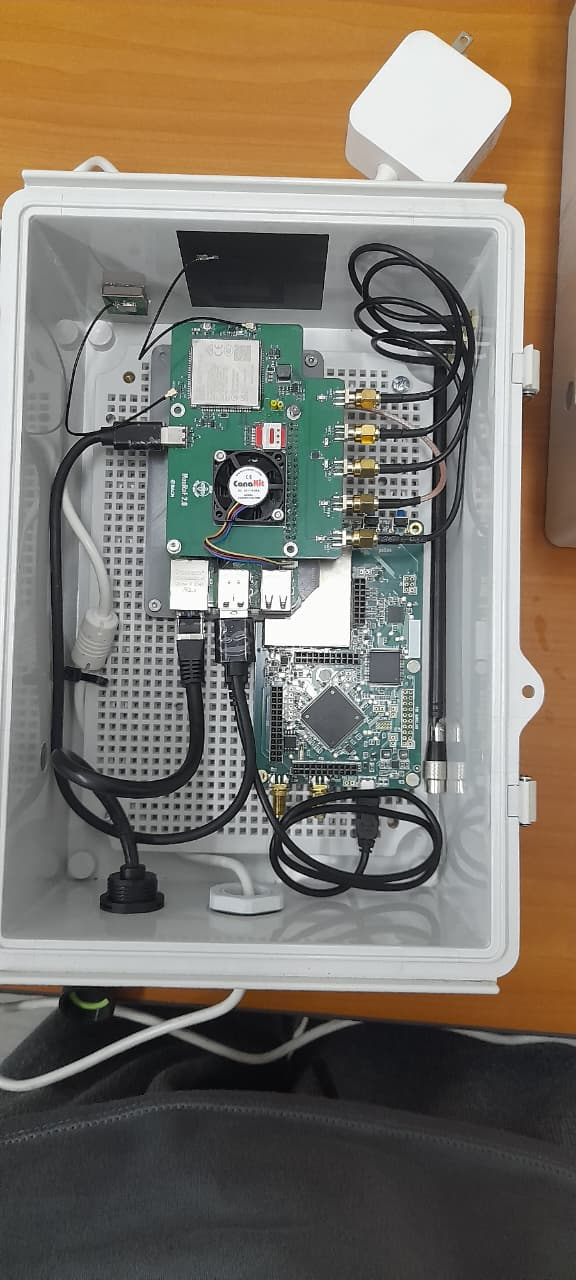
\includegraphics[width=0.55\textwidth]{section/img/cap04_hw/product.jpeg}
    \caption{Vista del conjunto físico del nodo ANE2. Fuente: elaboración propia.}
    \label{fig:hw_producto_ane2}
\end{figure}

\begin{figure}[H]
\centering
\setlength{\fboxsep}{4pt}
\scriptsize
\begin{tabular}{@{}c c c c c@{}}
\fbox{\begin{minipage}{0.14\textwidth}\centering Antenas\\TDT\\VHF/UHF\\$>2$ GHz\end{minipage}} &
$\rightarrow$ &
\fbox{\begin{minipage}{0.17\textwidth}\centering MonRaF2\\filtros\\mux RF\\LTE/GNSS\end{minipage}} &
$\rightarrow$ &
\fbox{\begin{minipage}{0.15\textwidth}\centering HackRF One\\IQ por USB\end{minipage}} \\
&&&& $\downarrow$ \\
\fbox{\begin{minipage}{0.15\textwidth}\centering Fuente externa\\5 V con margen\end{minipage}} &
$\rightarrow$ &
\fbox{\begin{minipage}{0.17\textwidth}\centering Raspberry Pi 5\\control\\telemetría\\procesamiento\end{minipage}} &
$\rightarrow$ &
\fbox{\begin{minipage}{0.15\textwidth}\centering Plataforma\\campañas\\reportes\end{minipage}}
\end{tabular}
\caption{Diagrama de bloques de hardware del nodo de sensado. Fuente: elaboración propia.}
\label{fig:hw_diagrama_bloques}
\end{figure}

\section{Desarrollo técnico}

\subsection{Trazabilidad contra requerimientos ANE}

La Tabla~\ref{tab:hw_trazabilidad_requisitos} relaciona los requerimientos
finales del sistema que dependen del hardware con los elementos físicos que los
soportan. La columna de estado usa cuatro marcas: implementado, parcial,
pendiente y recomendado. Esta clasificación separa lo existente en el prototipo de
lo que debe endurecerse para una versión de campo.

\scriptsize
\setlength{\tabcolsep}{3pt}
\begin{longtable}{@{}p{1.2cm} p{4.3cm} p{4.8cm} p{1.9cm}@{}}
\caption{Trazabilidad de requisitos ANE contra capacidades de hardware.}
\label{tab:hw_trazabilidad_requisitos}\\
\toprule
\textbf{ID} & \textbf{Requerimiento final asociado} & \textbf{Implementación o evidencia técnica en el nodo} & \textbf{Estado} \\
\midrule
\endfirsthead
\toprule
\textbf{ID} & \textbf{Requerimiento final asociado} & \textbf{Implementación o evidencia técnica en el nodo} & \textbf{Estado} \\
\midrule
\endhead
3.1.1 & Integrar conexión móvil mediante SIM institucional para transmisión de datos, sin depender de tecnologías propietarias, y mejorar la precisión horizontal y vertical con GNSS civil L1. & SIM7600G-H aporta LTE Cat-4, ranura nano SIM y GNSS multiconstelación. La ubicación queda disponible para georreferenciación y el enlace celular actúa como canal de datos cuando no hay red fija. & Parcial \\
3.2.1 & Agregar una tarjeta que permita usar cuatro antenas distintas en procesos de adquisición espectral. & MonRaF2 concentra puertos SMA, rutas MAIN/GNSS/AUX, filtros, conmutación RF y control GPIO desde la Raspberry Pi. La ruta documentada cubre TDT, VHF/UHF y $>2$ GHz; la cuarta posición queda reservada para expansión. & Parcial \\
3.2.2 & Agregar a cada sensor un kit de tres antenas específicas para recepción: TDT, $f>2$ GHz para telefonía móvil y VHF/UHF con frecuencias intermedias. & El montaje físico separa antenas por banda objetivo, conserva conectores de 50~$\Omega$ y registra la antena seleccionada durante la campaña de medición. & Implementado \\
3.3.1 & Optimizar la compatibilidad electromagnética para reducir interferencias que puedan falsear las mediciones espectrales del SDR. & El diseño contempla gabinete, separación de rutas RF y digitales, sellado, protección ESD, filtrado y selección de sitio. Falta campaña formal de susceptibilidad e inmunidad. & Parcial \\
4.1.1 & Sincronizar cada sensor con reloj de red NTP para etiquetado temporal de muestreos. & NTP depende del canal IP disponible y GNSS aporta posición y referencia de sitio. La verificación de sello temporal debe acompañar las campañas de captura. & Parcial \\
4.1.2 & Incluir calibración de frecuencia, ganancia de recepción, balance IQ y corrección de offset, con verificación mediante equipos certificados. & Existen mediciones operativas y análisis de balance IQ. La calibración trazable con instrumento certificado queda como requisito de cierre metrológico. & Pendiente \\
4.2.1 & Determinar el DANL, entendido como el nivel más bajo de señal detectable en ausencia de señal presente. & La caracterización requiere medición controlada del piso de ruido por banda, antena, ganancia y ancho de banda configurado. & Pendiente \\
4.2.2 & Determinar el rango dinámico entre la señal más grande medible sin distorsión y la señal mínima detectable sobre el ruido. & HackRF One usa ADC de 8 bits y requiere control estricto de ganancia para evitar saturación; falta barrido formal con señales patrón. & Pendiente \\
4.2.3 & Determinar la exactitud de frecuencia como diferencia máxima aceptable entre la frecuencia real y la medida por el equipo. & La exactitud se debe validar con fuente RF certificada y registro de offset por configuración de muestreo. & Pendiente \\
4.2.4 & Determinar la precisión de amplitud como margen de error en la medición de potencia de una señal, expresado en dB. & La cadena antena, mux, filtros, cables y HackRF requiere presupuesto de pérdidas y comparación contra instrumento patrón. & Pendiente \\
\bottomrule
\end{longtable}
\setlength{\tabcolsep}{6pt}
\normalsize

\subsection{Arquitectura física del nodo}

El nodo se compone de una Raspberry Pi 5, una tarjeta HackRF One y una PCB
MonRaF2. La Raspberry Pi 5 coordina la ejecución de software, el HackRF One
realiza la recepción SDR y MonRaF2 concentra conectividad, geolocalización,
señales de control, protecciones y rutas RF.

\begin{table}[H]
\centering
\caption{Inventario funcional de componentes de hardware del nodo ANE2.}
\label{tab:hw_inventario}
\begin{tabularx}{\textwidth}{>{\bfseries}p{3.1cm} p{3.1cm} X}
\toprule
Componente & Función principal & Criterio de integración \\
\midrule
Raspberry Pi 5 & Computador de borde & Ejecuta control, telemetría, adquisición, procesamiento y comunicación. No debe tratarse como fuente principal para todos los periféricos en una versión robusta. \\
HackRF One & Receptor SDR & Digitaliza señales RF como muestras IQ. Debe recibir la ruta RF ya seleccionada/acondicionada y requiere una alimentación estable para evitar fallas bajo carga. \\
MonRaF2 & Tarjeta de integración & Integra LTE/GNSS, UART/USB/GPIO, protecciones, filtros y una ruta RF con función tipo mux/switch. Es el punto de terminación de antenas y control de rutas RF. \\
SIM7600G-H & LTE/GNSS & Proporciona datos celulares y ubicación. Su consumo y transitorios deben considerarse dentro del árbol de potencia. \\
Antenas RF, LTE y GNSS & Interfaz electromagnética & Se conectan al subsistema de MonRaF2. La conexión no debe documentarse como antena directa al HackRF, porque el diseño incluye una etapa de selección/acondicionamiento RF. \\
Fuente y gabinete & Energía y protección física & La fuente debe proveer margen de corriente; el gabinete debe proteger el montaje, conservar ventilación y sellar puntos vulnerables como alimentación y coaxiales. \\
\bottomrule
\end{tabularx}
\end{table}

La Figura~\ref{fig:hw_modulos_principales} muestra los tres módulos principales
del nodo. Su separación ayuda a diagnosticar fallas: no es lo mismo un problema
de ruta RF, de alimentación, de procesamiento, de enlace celular o de ubicación.

\begin{figure}[H]
    \centering
    \begin{subfigure}{0.31\textwidth}
        \centering
        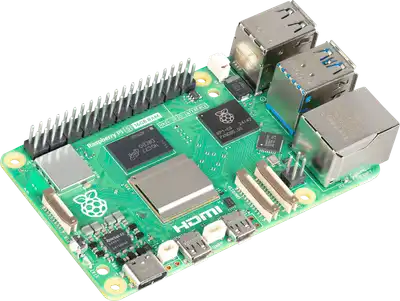
\includegraphics[width=\textwidth]{section/img/cap04_hw/rpi5.png}
        \caption{Raspberry Pi 5.}
    \end{subfigure}
    \hfill
    \begin{subfigure}{0.31\textwidth}
        \centering
        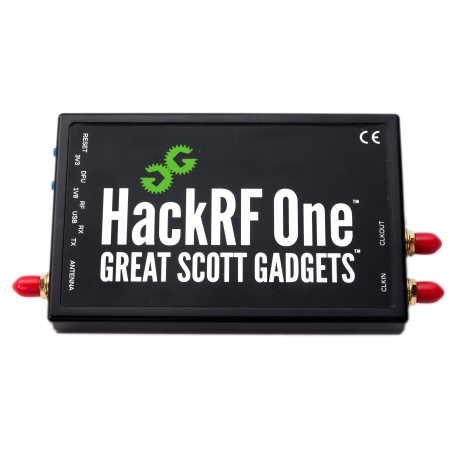
\includegraphics[width=\textwidth]{section/img/cap04_hw/hackrfone.jpeg}
        \caption{HackRF One.}
    \end{subfigure}
    \hfill
    \begin{subfigure}{0.31\textwidth}
        \centering
        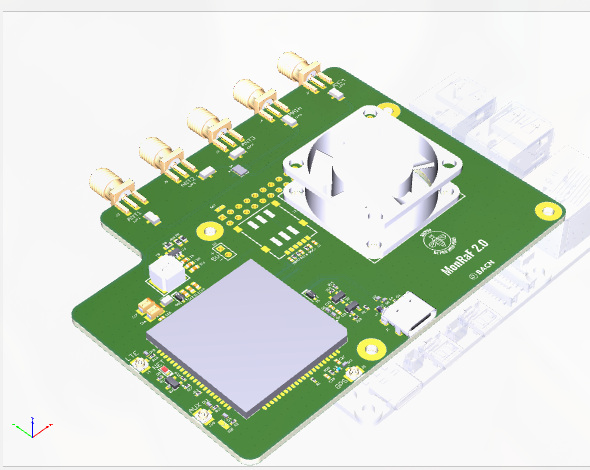
\includegraphics[width=\textwidth]{section/img/cap04_hw/monraf2-default.jpeg}
        \caption{MonRaF2.}
    \end{subfigure}
    \caption{Módulos principales del hardware ANE2. Fuente: elaboración propia.}
    \label{fig:hw_modulos_principales}
\end{figure}

\subsection{Fichas técnicas de componentes}

\scriptsize
\setlength{\tabcolsep}{3pt}
\begin{longtable}{@{}p{2.4cm} p{3.5cm} p{5.2cm} p{1.7cm}@{}}
\caption{Fichas técnicas resumidas de los elementos de hardware.}
\label{tab:hw_fichas}\\
\toprule
\textbf{Elemento} & \textbf{Parámetros relevantes} & \textbf{Rol dentro de ANE2} & \textbf{Estado} \\
\midrule
\endfirsthead
\toprule
\textbf{Elemento} & \textbf{Parámetros relevantes} & \textbf{Rol dentro de ANE2} & \textbf{Estado} \\
\midrule
\endhead
Raspberry Pi 5 & ARM Cortex-A76 de cuatro núcleos, RAM de 8 GB, USB 3.0, GPIO, Ethernet/WiFi & Computador de borde para adquisición, procesamiento, telemetría, control RF y comunicación con la plataforma. & Implementado \\
HackRF One & 1 MHz--6 GHz, hasta 20 MHz de ancho instantáneo, ADC de 8 bits, LNA 0--40 dB, VGA 0--62 dB & Receptor SDR principal; entrega muestras IQ y permite campañas de monitoreo multibanda. & Implementado \\
MonRaF2 & PCB de integración con puertos SMA, rutas RF, filtros, mux/switch, GPIO, UART/USB, SIM7600G-H y protecciones & Concentra antenas, conectividad celular, GNSS, control auxiliar y adaptación de rutas hacia el receptor. & Implementado \\
SIM7600G-H & LTE Cat-4, LTE-FDD/TDD, GSM/GPRS/EDGE, WCDMA/HSPA+, USB 2.0, UART, GNSS multiconstelación & Enlace celular de datos, registro de red, ubicación y soporte de sincronización operacional. & Implementado \\
Antena TDT & 470--698 MHz, recepción UHF, adaptación a SMA, ganancia típica 5--7.5 dBi & Recepción de televisión digital terrestre y pruebas RMTDT. & Implementado \\
Antena VHF/UHF & 25 MHz--1.3 GHz, 50~$\Omega$, adaptadores SO239--SMA/BNC, ganancia promedio cercana a 3.5 dBi & Monitoreo de VHF, UHF, FM y frecuencias intermedias. & Implementado \\
Antena $>2$ GHz & 600--960 MHz y 1710--6000 MHz, 50~$\Omega$, SMA macho, ganancia máxima cercana a 6 dBi & Cobertura de bandas móviles, LTE/5G sub-6 y servicios de microondas. & Implementado \\
Fuente & 5 V DC por USB-C, adaptador recomendado de 45 W, reserva para cargas SDR/LTE & Alimentación del nodo; debe evolucionar a rieles medibles y distribuidos para campo. & Parcial \\
Gabinete & Protección ambiental tipo IP68 en chasis, sellado externo de alimentación, separación de antenas y ventilación & Protección mecánica, instalación en campo y reducción de exposición a polvo, humedad e interferencias. & Parcial \\
\bottomrule
\end{longtable}
\setlength{\tabcolsep}{6pt}
\normalsize

\subsection{Antenas y montaje mecánico}

El kit de antenas se organiza por banda de trabajo: TDT para UHF de televisión,
VHF/UHF para monitoreo amplio y una antena de alta frecuencia para bandas
móviles y servicios por encima de 2 GHz. Esta separación evita exigir a una sola
antena un comportamiento plano en todo el rango del HackRF y facilita que la
plataforma seleccione puerto y preajuste según la campaña.

La caracterización disponible muestra que la antena VHF/UHF tiene mejor
comportamiento entre 200 MHz y 600 MHz, con degradación progresiva por encima
de 1 GHz. La antena TDT mantiene adaptación aceptable en la banda UHF de
televisión, con mínimos de SWR en frecuencias clave de la banda. Para antenas
referenciadas a tierra, el plano de tierra no es un accesorio: mejora la
adaptación, estabiliza resonancias y reduce potencia reflejada.

\begin{figure}[H]
    \centering
    \begin{subfigure}{0.48\textwidth}
        \centering
        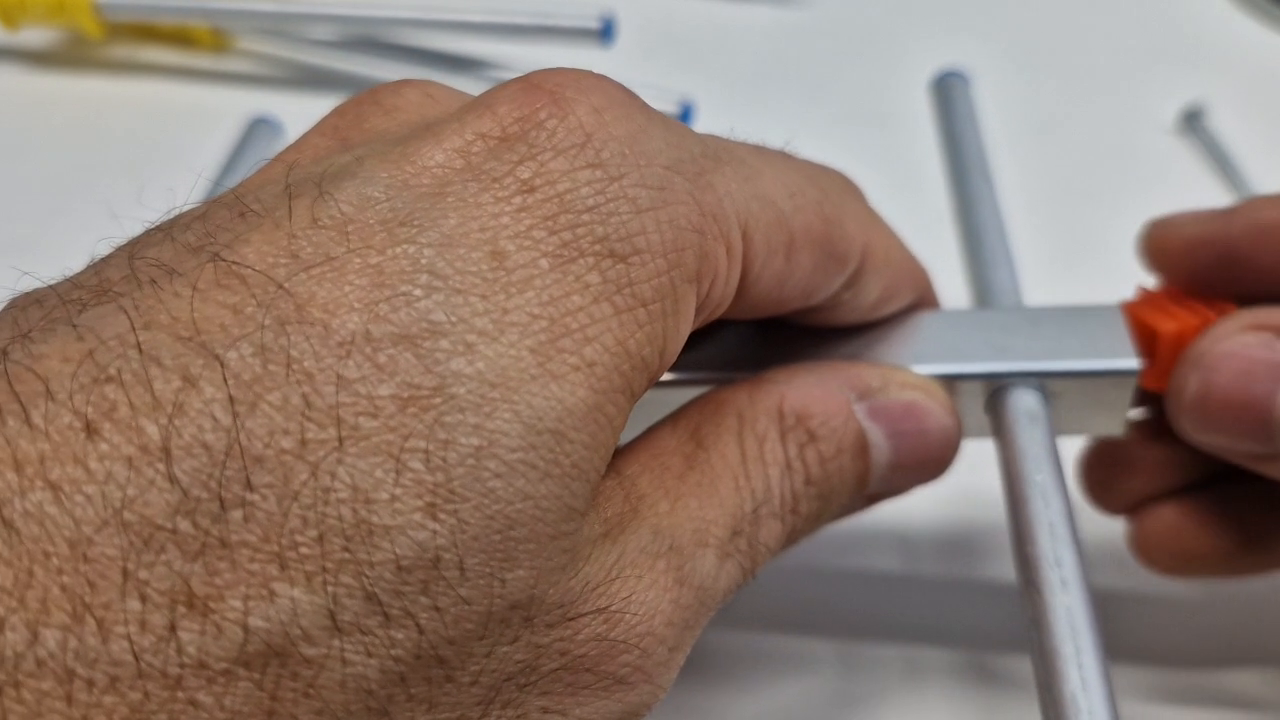
\includegraphics[width=\textwidth]{section/img/cap04_hw/antena_tdt_elemento.png}
        \caption{Alineación de elemento en antena TDT.}
    \end{subfigure}
    \hfill
    \begin{subfigure}{0.48\textwidth}
        \centering
        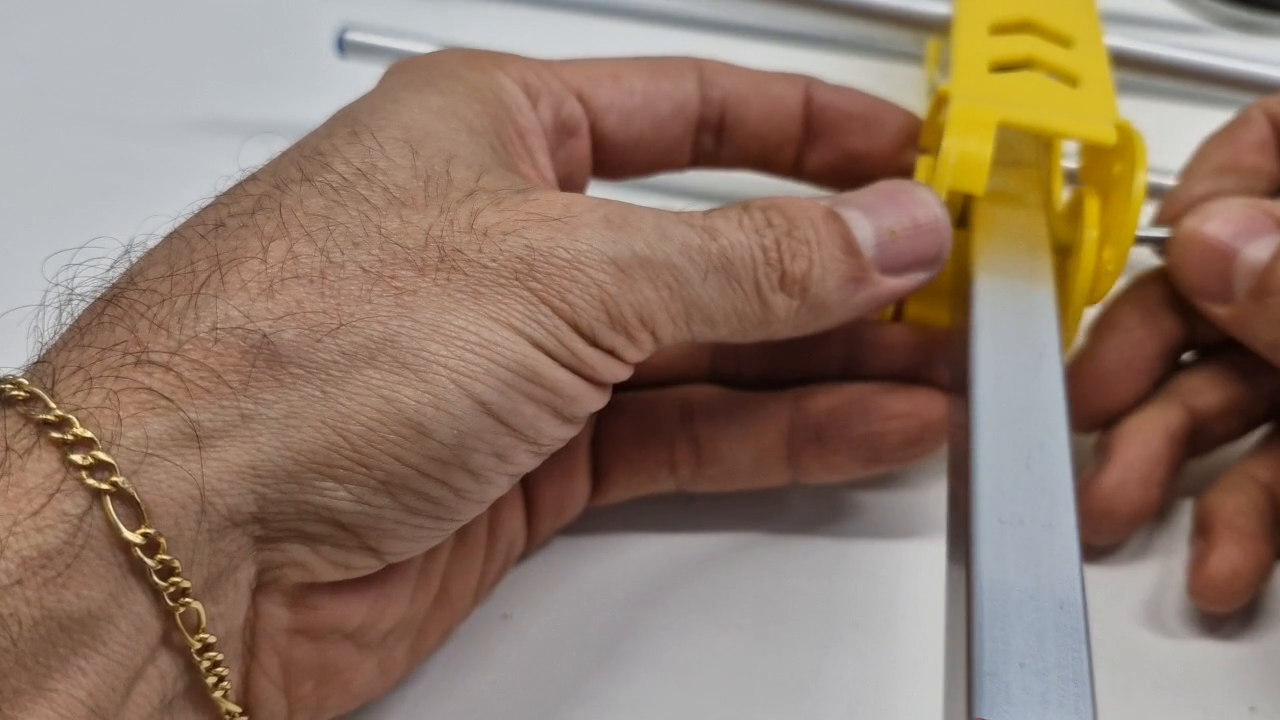
\includegraphics[width=\textwidth]{section/img/cap04_hw/antena_tdt_soporte.png}
        \caption{Fijación del soporte direccional TDT.}
    \end{subfigure}
    \caption{Puntos críticos de ensamble de la antena TDT. Fuente: elaboración propia.}
    \label{fig:hw_antena_tdt_ensamble}
\end{figure}

\begin{figure}[H]
    \centering
    \begin{subfigure}{0.48\textwidth}
        \centering
        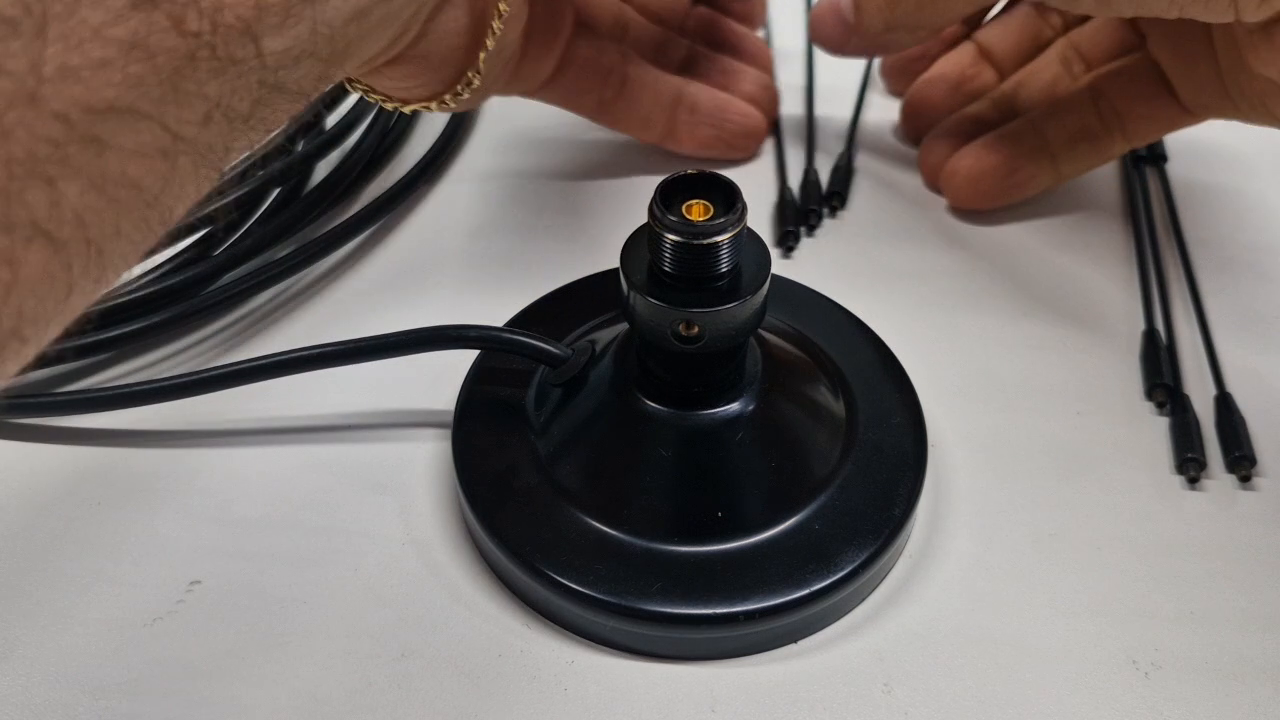
\includegraphics[width=\textwidth]{section/img/cap04_hw/antena_vhfuhf_base.png}
        \caption{Base magnética y puerto de conexión.}
    \end{subfigure}
    \hfill
    \begin{subfigure}{0.48\textwidth}
        \centering
        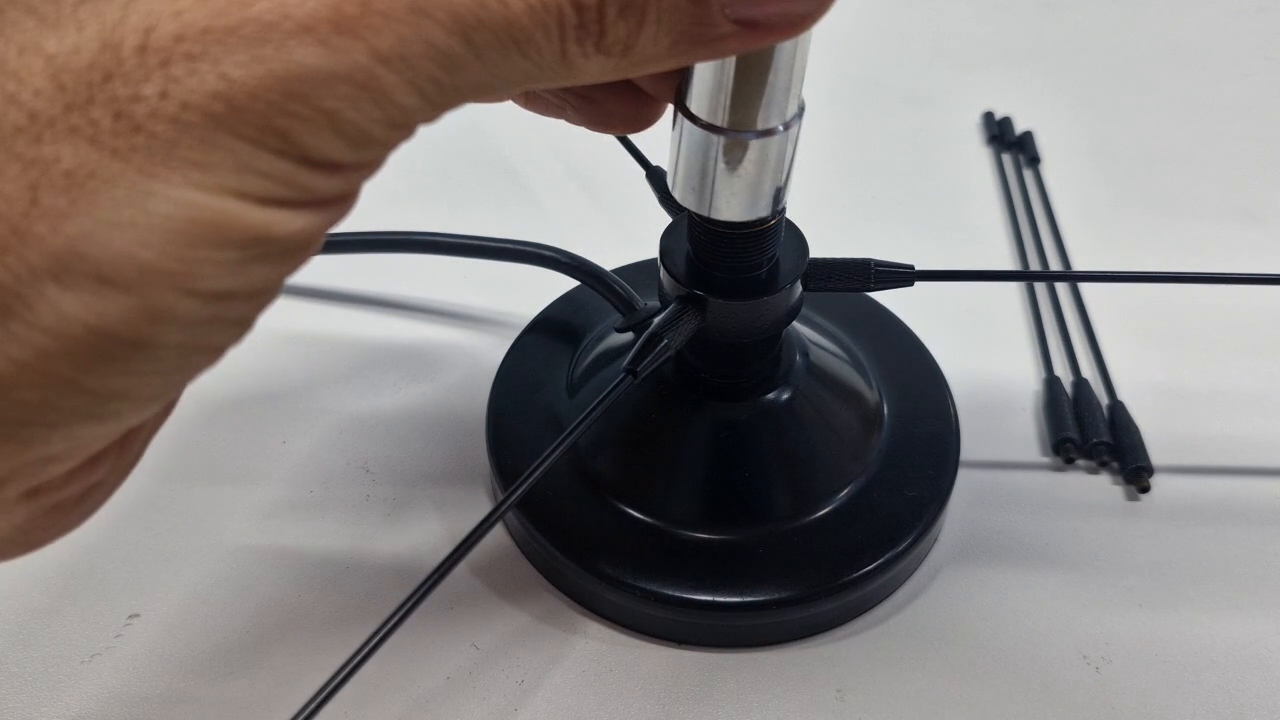
\includegraphics[width=\textwidth]{section/img/cap04_hw/antena_vhfuhf_radiales.png}
        \caption{Instalación de radiales y elemento vertical.}
    \end{subfigure}
    \caption{Puntos críticos de ensamble de la antena VHF/UHF. Fuente: elaboración propia.}
    \label{fig:hw_antena_vhfuhf_ensamble}
\end{figure}

\subsection{Ruta RF, puertos, filtros, mux y pérdidas}

La ruta RF no debe describirse como una antena conectada directamente al HackRF.
El esquemático de MonRaF2 muestra redes de antena como \texttt{MAIN\_ANT},
\texttt{GNSS\_ANT} y \texttt{AUX\_ANT}, además de conectores RF, filtros LPF y
una etapa de conmutación/mux RF controlada por señales GPIO. En términos
operativos, MonRaF2 actúa como la tarjeta que recibe y ordena las rutas de
antena antes de que la señal sea usada por el subsistema de adquisición o por
el módulo celular/GNSS.

El flujo físico recomendado queda entonces:

\begin{enumerate}[leftmargin=*]
    \item Las antenas externas se conectan a puertos SMA de MonRaF2.
    \item MonRaF2 selecciona, protege o acondiciona rutas RF mediante su red de
    filtros, conectores y mux/switch RF.
    \item La ruta RF seleccionada alimenta el subsistema correspondiente:
    adquisición SDR, LTE o GNSS, según el modo de operación.
    \item La Raspberry Pi 5 controla la operación y recibe los datos del HackRF
    por USB, pero no debe asumirse como concentrador físico de antenas.
\end{enumerate}

\begin{figure}[H]
    \centering
    \includegraphics[page=3,width=0.92\textwidth,height=0.72\textheight,keepaspectratio]{section/img/cap04_hw/monraf2-schematics.pdf}
    \caption{Detalle esquemático de rutas RF, filtros y etapa tipo mux/switch en MonRaF2. Fuente: elaboración propia.}
    \label{fig:hw_monraf2_rf}
\end{figure}

\begin{table}[H]
\centering
\caption{Presupuesto cualitativo de ruta RF y puntos de pérdida.}
\label{tab:hw_rf_budget}
\begin{tabularx}{\textwidth}{>{\bfseries}p{3.2cm} p{3cm} X}
\toprule
Tramo & Pérdida o restricción & Criterio de control \\
\midrule
Antena a coaxial & Adaptación de impedancia y conectores & Mantener 50~$\Omega$ en la cadena de medición; cuando la antena original sea 75~$\Omega$, usar adaptación hacia SMA. \\
Coaxial y adaptadores & Pérdida por longitud, transición y apriete & Usar cables cortos, conectores firmes y verificación visual antes de cada campaña. \\
Puerto SMA de MonRaF2 & Selección física de antena & Registrar puerto/antena en la plataforma para no confundir una medición de banda con otra. \\
Filtros LPF y protección & Limitación de banda y protección de entrada & Validar que el filtro corresponde a la ruta seleccionada y que no bloquea la banda objetivo. \\
Mux/switch RF & Pérdida típica de inserción cercana a 1.25 dB & Incluir esta pérdida en el margen de sensibilidad y mantener GPIO en el estado correcto. \\
Entrada HackRF & Saturación y piso de ruido & Ajustar LNA/VGA por escenario; conservar la configuración durante comparaciones. \\
LTE/GNSS & Separación de rutas y antenas & Evitar que transmisión celular o mala ubicación GNSS contaminen mediciones de RF. \\
\bottomrule
\end{tabularx}
\end{table}

\subsection{GPS/GNSS y conectividad LTE}

El módulo SIM7600G-H cumple dos funciones distintas: comunicación celular y
georreferenciación. En conectividad, soporta GSM/GPRS/EDGE, WCDMA/HSPA+ y
LTE-FDD/LTE-TDD, con categoría LTE Cat-4 de hasta 150 Mbps de bajada y
50 Mbps de subida en condiciones ideales de red. En ubicación, soporta GPS,
GLONASS, BeiDou, Galileo y QZSS, con salida NMEA por UART o USB según la
configuración.

La operación correcta de GNSS no depende solamente del módulo. La antena debe
tener vista despejada al cielo, evitar techos de losa, marquesinas, árboles
densos y superficies metálicas cercanas, y conservar un cono de visibilidad
amplio hacia el cenit. Para disminuir multipath e interferencia, el sitio debe
mantener separación frente a antenas transmisoras de alta potencia y evitar
fachadas metálicas o vidrios extensos que reflejen señales satelitales.

La conectividad LTE debe validarse como una condición de sitio, no como una
propiedad fija del hardware. Antes de dejar un nodo operativo se debe confirmar
señal celular suficiente, estabilidad de túnel o canal IP, estado de la SIM,
registro de red y comportamiento de LED del módem. Para despliegue, una señal
RSRP mayor a -95 dBm es un criterio práctico de aceptación inicial.

\subsection{Árbol de potencia y gestión térmica}

El principal aprendizaje del hardware es que el diseño de potencia debe
preceder al diseño mecánico y de software. En las primeras integraciones, gran
parte de la energía de periféricos se entregaba desde la Raspberry Pi 5. Ese
enfoque funciona para pruebas de bajo alcance, pero se vuelve frágil cuando se
combinan SDR, LTE, GNSS, procesamiento sostenido y tráfico de red.

La evidencia de telemetría muestra tres hechos prácticos:

\begin{itemize}[leftmargin=*]
    \item Las pruebas con HackRF y peticiones desde servidor elevaron la
    temperatura del procesador hasta el orden de 75 $^\circ$C.
    \item El riel EXT5V presentó caídas bajo cargas pesadas, aun cuando no
    todas las corridas terminaron marcando una bandera persistente de
    subtensión.
    \item Las pruebas con alimentación externa para periféricos tuvieron mejor
    margen para sostener carga combinada.
\end{itemize}

Por ello, el criterio para un nuevo producto o una siguiente versión debe ser:

\begin{quote}
El nodo debe tener un árbol de potencia externo y generoso, con capacidad para
la carga actual y para extensiones futuras. La Raspberry Pi 5 debe ser tratada
como carga y controlador, no como fuente primaria para el resto del sistema.
\end{quote}

\begin{table}[H]
\centering
\caption{Presupuesto de potencia y térmico para operación del nodo.}
\label{tab:hw_power_thermal_budget}
\begin{tabularx}{\textwidth}{>{\bfseries}p{3.2cm} p{3.2cm} X}
\toprule
Elemento & Demanda o riesgo & Criterio de diseño \\
\midrule
Raspberry Pi 5 & Carga de CPU, USB y red; límite térmico operativo & Tratarla como carga crítica, mantener ventilación y evitar superar 85 $^\circ$C en reposo post-instalación. \\
HackRF One & Consumo sostenido durante captura IQ y presión sobre USB & Alimentación estable y separación de riel frente a cargas pulsantes. \\
SIM7600G-H & Transitorios de red celular y registro LTE & Reservar margen de corriente y desacople cerca del módulo. \\
Mux RF y GPIO & Carga baja, pero sensible a estados lógicos incorrectos & Alimentar desde riel lógico estable y registrar estado de selección. \\
Antenas activas o futuras extensiones & Consumo adicional no siempre presente & Dejar reserva de potencia para expansión sin rediseño completo. \\
Gabinete & Retención térmica y sellado & Combinar protección ambiental con ventilación o disipación; no encerrar el nodo sin camino térmico. \\
\bottomrule
\end{tabularx}
\end{table}

\begin{table}[H]
\centering
\caption{Criterios mínimos para una versión robusta del árbol de potencia.}
\label{tab:hw_power_tree}
\begin{tabularx}{\textwidth}{>{\bfseries}p{3.4cm} X}
\toprule
Criterio & Implicación de diseño \\
\midrule
Fuente principal sobredimensionada & Debe alimentar simultáneamente Raspberry Pi 5, HackRF, MonRaF2, LTE/GNSS y periféricos futuros sin operar en el límite. \\
Rieles distribuidos & Las cargas de alto consumo o con transitorios, como SDR y LTE, deben alimentarse desde rieles dedicados o reguladores con margen, no desde el puerto de la Raspberry Pi. \\
Medición de rieles & El sistema debe conservar telemetría de voltaje, corriente, temperatura y eventos de subtensión para diagnóstico. \\
Protección y desacople & Se deben incluir protecciones, filtrado y capacitancia local cerca de cargas ruidosas o pulsantes. \\
Reserva para extensiones & El diseño debe contemplar nuevos servicios, antenas, sensores, almacenamiento o comunicaciones sin rediseñar la alimentación desde cero. \\
\bottomrule
\end{tabularx}
\end{table}

\subsection{Compatibilidad electromagnética}

El hardware de ANE2 comparte en un mismo volumen físico recepción sensible,
procesamiento digital, USB, LTE, GNSS y alimentación conmutada. Por esa razón,
la compatibilidad electromagnética no puede tratarse como revisión estética del
gabinete: afecta directamente la confiabilidad de las mediciones.

\begin{table}[H]
\centering
\caption{Medidas de mitigación EMC y pruebas mínimas.}
\label{tab:hw_emc}
\begin{tabularx}{\textwidth}{>{\bfseries}p{3cm} p{4.4cm} X}
\toprule
Riesgo & Mitigación & Prueba mínima \\
\midrule
Acoplamiento LTE sobre RF & Separar físicamente antena LTE/GNSS de entrada SDR y conservar coaxiales cortos. & Comparar piso de ruido con LTE inactivo, registrado y transmitiendo. \\
Multipath GNSS & Evitar metal, vidrio extenso y obstrucciones sobre la antena GNSS. & Verificar fix con al menos 4 satélites y coordenadas coherentes con el sitio. \\
Ruido de fuente conmutada & Usar desacople local, ferritas cuando aplique y rieles separados para cargas pulsantes. & Medir estabilidad de EXT5V y observar cambios en PSD con distintas cargas. \\
ESD y manipulación de antenas & Mantener protección de entrada, conectores firmes y manipulación con equipo apagado. & Inspección de continuidad, apriete y ausencia de daño antes de energizar. \\
Encierro térmico & No instalar en caja estanca sin disipación o ventilación natural. & Verificar temperatura en reposo y bajo adquisición sostenida. \\
\bottomrule
\end{tabularx}
\end{table}

\section{Entradas, salidas e interfaces}

\begin{table}[H]
\centering
\caption{Interfaces principales del hardware ANE2.}
\label{tab:hw_interfaces}
\begin{tabularx}{\textwidth}{>{\bfseries}p{3cm} p{3cm} X}
\toprule
Interfaz & Tipo & Contrato operacional \\
\midrule
Antenas a MonRaF2 & RF coaxial & Las antenas se conectan a MonRaF2. La etapa RF de la tarjeta selecciona o acondiciona rutas antes de la adquisición o uso LTE/GNSS. \\
MonRaF2 a HackRF & RF seleccionado & El HackRF debe recibir una ruta RF controlada, no una conexión de antena asumida como directa. \\
HackRF a Raspberry Pi 5 & USB & Transporta muestras IQ y comandos de configuración. El \textit{sample rate} aumenta simultáneamente el ancho instantáneo y la presión sobre USB/CPU. \\
Raspberry Pi 5 a MonRaF2 & GPIO, UART, USB & Permite control auxiliar, comunicación con LTE/GNSS y señales de estado. \\
MonRaF2 a red celular & LTE & Provee conectividad de datos para estado, mediciones, campañas y reintentos. \\
MonRaF2 a GNSS & GNSS/GPS & Entrega ubicación del nodo para reportes y trazabilidad de mediciones. \\
Fuente externa a cargas & DC regulado & Debe distribuir potencia a Raspberry Pi 5, HackRF, MonRaF2 y expansiones con margen suficiente. \\
\bottomrule
\end{tabularx}
\end{table}

\section{Decisiones de diseño o implementación}

\small
\begin{longtable}{p{3cm} p{4cm} p{5.2cm}}
\caption{Decisiones de diseño de hardware y justificación.}
\label{tab:hw_decisiones}\\
\toprule
\textbf{Decisión} & \textbf{Justificación} & \textbf{Implicación práctica} \\
\midrule
\endfirsthead
\toprule
\textbf{Decisión} & \textbf{Justificación} & \textbf{Implicación práctica} \\
\midrule
\endhead
Usar MonRaF2 como concentrador RF y de conectividad & La tarjeta contiene rutas de antena, filtros, mux/switch RF, LTE/GNSS y señales de control. & Las antenas se documentan y cablean hacia MonRaF2; el HackRF queda como receptor SDR dentro de la cadena, no como punto directo de antena. \\
Usar Raspberry Pi 5 como computador de borde & Tiene capacidad suficiente para orquestación, telemetría y control del SDR. & Debe protegerse de sobrecarga eléctrica; no debe alimentar todos los periféricos en una versión robusta. \\
Usar HackRF One como receptor SDR & Permite recepción flexible por software y adquisición IQ. & Requiere ganancia configurada con criterio y alimentación estable. \\
Separar potencia de control & Los problemas de subtensión aparecen cuando la distribución de energía queda demasiado acoplada a la Raspberry Pi. & El árbol de potencia externo pasa a ser requisito de producto. \\
Mantener telemetría de salud & Temperatura, voltajes, corrientes y banderas de \textit{throttling} permiten diagnosticar fallas reales. & Cada prueba de RF o conectividad debe acompañarse de telemetría eléctrica. \\
Usar antenas por banda & Las antenas no son verdaderamente planas en todo el rango del SDR. & La plataforma y el operador deben seleccionar la antena adecuada para cada campaña. \\
\bottomrule
\end{longtable}
\normalsize

\section{Problemas presentados y ajustes realizados}

\scriptsize
\setlength{\tabcolsep}{3pt}
\begin{longtable}{@{}p{1.9cm} p{2.6cm} p{2.6cm} p{3cm} p{2.1cm}@{}}
\caption{Problemas presentados, decisiones y ajustes realizados en hardware.}
\label{tab:hw_problemas}\\
\toprule
\textbf{Problema} & \textbf{Evidencia} & \textbf{Causa probable} & \textbf{Decisión o ajuste} & \textbf{Resultado} \\
\midrule
\endfirsthead
\toprule
\textbf{Problema} & \textbf{Evidencia} & \textbf{Causa probable} & \textbf{Decisión o ajuste} & \textbf{Resultado} \\
\midrule
\endhead
Subtensión y bajo margen de potencia & Caídas de EXT5V bajo cargas SDR/LTE y escenarios con eventos de alimentación insuficiente. & Demasiadas cargas alimentadas o condicionadas desde la Raspberry Pi 5. & Diseñar un árbol de potencia externo, generoso y medible. & Requisito obligatorio para una versión robusta. \\
Aumento de temperatura bajo carga & Pruebas con HackRF y peticiones desde servidor alcanzaron temperaturas cercanas a 75 $^\circ$C. & Procesamiento sostenido, actividad USB y carga RF/LTE simultánea. & Mantener disipación, ventilación y telemetría de temperatura. & La temperatura queda como restricción operativa. \\
Ambigüedad en ruta de antenas & El diseño incluye redes MAIN/GNSS/AUX, filtros y mux/switch RF en MonRaF2. & Interpretar la antena como conexión directa al HackRF simplifica de forma incorrecta la cadena RF. & Documentar MonRaF2 como entrada y selección RF. & La conexión física queda alineada con el esquemático. \\
Dependencia del enlace LTE & Las pruebas de campo usan conectividad celular para operación y envío de datos. & La red celular puede variar por cobertura, antena, SIM y ubicación. & Separar diagnóstico de RF, cómputo, potencia y LTE. & Las fallas se pueden atribuir con mejor evidencia. \\
Riesgo de saturación RF & HackRF no usa AGC de hardware en esta cadena de operación. & Ganancia excesiva o emisores fuertes pueden saturar el ADC de 8 bits. & Ajustar ganancia por escenario y conservar configuraciones durante comparaciones. & Menor riesgo de confundir artefactos con emisiones reales. \\
Adaptación de antenas & VHF/UHF, TDT y $>2$ GHz tienen bandas óptimas distintas. & Una antena única no cubre con buen desempeño todo el rango 1 MHz--6 GHz. & Mantener kit por banda y registrar puerto/antena en campaña. & Mejor trazabilidad entre medición, banda y condición física. \\
\bottomrule
\end{longtable}
\setlength{\tabcolsep}{6pt}
\normalsize

\section{Validación, pruebas o evidencias}

La validación usada para esta sección combina inspección de esquemático,
fotografías del montaje, ensamble de antenas, caracterización de antenas,
pruebas de aceptación funcional y telemetría de nodos bajo reposo, carga SDR,
carga LTE y carga combinada. Los indicadores más útiles fueron temperatura ARM,
EXT5V, corrientes de rieles, banderas de subtensión, frecuencia de CPU y estados
de \textit{throttling}.

\begin{table}[H]
\centering
\caption{Resumen de telemetría eléctrica y térmica inspeccionada.}
\label{tab:hw_telemetria}
\begin{tabularx}{\textwidth}{>{\bfseries}p{3cm} p{2.4cm} p{2.1cm} p{1.4cm} X}
\toprule
Escenario & Temperatura ARM & EXT5V & UV & Lectura para operación \\
\midrule
Nodo en reposo & 54.3--57.6 $^\circ$C & 5.006--5.041 V & No & Referencia base con sistema operativo y telemetría. \\
HackRF en carga alta & 54.9--74.7 $^\circ$C & 4.748--4.965 V & No & La carga SDR aumenta demanda y temperatura. \\
Periféricos conectados en reposo & 45.0--52.1 $^\circ$C & 4.903--4.963 V & No & El margen mejora cuando no hay procesamiento pesado. \\
Petición media con periféricos & 61.5--75.7 $^\circ$C & 4.721--5.083 V & No & El sistema se acerca a límites térmicos y de alimentación. \\
Carga alta con periféricos externos & 49.4--75.2 $^\circ$C & 4.904--5.122 V & No & La alimentación externa mejora el margen frente a carga combinada. \\
\bottomrule
\end{tabularx}
\end{table}

\scriptsize
\setlength{\tabcolsep}{3pt}
\begin{longtable}{@{}p{1.15cm} p{2.35cm} p{2.45cm} p{2.45cm} p{2.9cm} p{1.8cm}@{}}
\caption{Protocolo de validación de hardware.}
\label{tab:hw_protocolo_validacion}\\
\toprule
\textbf{Req.} & \textbf{Condición de prueba} & \textbf{Instrumento o medio} & \textbf{Resultado observado} & \textbf{Criterio de aceptación} & \textbf{Estado} \\
\midrule
\endfirsthead
\toprule
\textbf{Req.} & \textbf{Condición de prueba} & \textbf{Instrumento o medio} & \textbf{Resultado observado} & \textbf{Criterio de aceptación} & \textbf{Estado} \\
\midrule
\endhead
3.1.1 & LTE de sitio & Panel de red, SIM y estado del módem & Registro de red y comunicación LTE cuando hay cobertura. & SIM institucional activa, canal estable por más de 10 minutos y RSRP mayor a -95 dBm. & Parcial \\
3.1.1 & GNSS de sitio & Coordenadas reportadas y condición de cielo abierto & El nodo reporta ubicación cuando la antena tiene visibilidad suficiente. & Coordenadas coherentes con sitio, lock de al menos 4 satélites y error dentro de la meta horizontal y vertical definida. & Parcial \\
3.2.1 & Inspección de ruta RF y multiplexación & Esquemático, revisión visual y tabla de puertos & MonRaF2 concentra MAIN/GNSS/AUX, filtros, mux RF y control GPIO. & Cada puerto debe mapearse a una banda, conmutar desde software y dejar reservada la cuarta ruta. & Parcial \\
3.2.2 & Ensamble de antena TDT & Inspección de boom, elementos y soporte & Elementos y soporte quedan fijados y alineados. & Sin piezas flojas, conector firme y orientación coherente con campaña TDT. & Implementado \\
3.2.2 & Ensamble de antena VHF/UHF & Inspección de base, radiales y elemento vertical & Base y radiales quedan instalados en el plano de referencia. & Radiales presentes, elemento vertical fijo y sin contacto accidental con metal externo. & Implementado \\
3.2.2 & Selección de antena por campaña & Prueba funcional de monitoreo & El usuario selecciona sensor online, puerto/antena y parámetros de ganancia. & El panel habilita adquisición, confirma configuración aplicada y conserva la antena usada en la evidencia. & Implementado \\
3.3.1 & EMC mínima & PSD comparativa, LTE activo/inactivo e inspección de sitio & Riesgo identificado por cercanía de antenas, fuente, cableado digital y gabinete. & Sin cambio anómalo de piso de ruido al activar LTE o cargas; separación física y puesta a tierra documentadas. & Recomendado \\
4.1.1 & Sello temporal de captura & Registro NTP y hora de adquisición & La hora depende de conectividad IP estable y configuración del sensor. & El muestreo debe quedar etiquetado con hora sincronizada antes de iniciar campaña. & Parcial \\
4.1.2 & Calibración de frecuencia, ganancia, IQ y offset & Generador RF, analizador o equipo certificado & Hay análisis IQ operativo; falta cierre con instrumento certificado. & Error de frecuencia, ganancia, balance IQ y offset dentro de tolerancia definida para el sensor. & Pendiente \\
4.2.1 & Medición DANL & Carga de 50~$\Omega$, configuración SDR y registro PSD & Pendiente de barrido formal por banda, ganancia y ancho de banda. & Piso de ruido documentado y repetible para cada condición de operación. & Pendiente \\
4.2.2 & Rango dinámico & Generador RF con barrido de potencia & Pendiente de determinar el punto de saturación y señal mínima útil. & Diferencia documentada entre señal máxima sin distorsión y señal mínima sobre DANL. & Pendiente \\
4.2.3 & Exactitud de frecuencia & Fuente RF certificada & Pendiente de comparación entre frecuencia patrón y frecuencia medida. & Error máximo de frecuencia documentado por banda y configuración. & Pendiente \\
4.2.4 & Precisión de amplitud & Instrumento patrón, presupuesto de pérdidas y señal conocida & Pendiente de compensar antena, cables, mux, filtros y ganancia SDR. & Error de potencia expresado en dB y trazado contra configuración de medición. & Pendiente \\
\bottomrule
\end{longtable}
\setlength{\tabcolsep}{6pt}
\normalsize

\section{Aprendizajes y transferencia de conocimiento}

\begin{itemize}[leftmargin=*]
    \item El árbol de potencia define la robustez del nodo. Si se alimentan
    periféricos exigentes desde la Raspberry Pi, el diseño queda sin margen.
    \item Las antenas pertenecen a la cadena de MonRaF2 y su etapa RF. El HackRF
    debe verse como receptor dentro de una ruta seleccionada, no como destino
    directo de todas las antenas.
    \item La telemetría eléctrica debe acompañar cualquier prueba RF. Sin
    voltajes, corrientes y temperatura es fácil confundir fallas de potencia con
    fallas de software.
    \item La caracterización de antenas debe leerse por banda. El plano de tierra
    y los adaptadores físicos cambian SWR, S11 y eficiencia real de recepción.
    \item La validación de campo debe separar sitio, potencia, RF, LTE y GNSS. Si
    se prueban juntos desde el inicio, las fallas quedan mezcladas.
    \item El diseño debe reservar margen para servicios futuros. Cada extensión
    de software o hardware aumenta demanda de energía, temperatura y tráfico.
\end{itemize}

\section{Limitaciones}

\begin{itemize}[leftmargin=*]
    \item Las cifras de telemetría resumen pruebas disponibles; no reemplazan una
    caracterización eléctrica completa con instrumentos de laboratorio.
    \item No se presentan curvas completas de consumo por banda, ganancia,
    temperatura ambiente, antena o ubicación.
    \item El diseño RF requiere validar pérdidas, aislamiento, adaptación de
    impedancias y compatibilidad electromagnética antes de una versión final de
    campo.
    \item La estabilidad LTE/GNSS depende de cobertura, antenas, SIM, ubicación y
    configuración del operador.
    \item La trazabilidad EMC está en estado parcial porque falta una campaña
    formal de susceptibilidad, inmunidad y emisiones conducidas/radiadas.
\end{itemize}

\section{Recomendaciones específicas}

\begin{enumerate}[leftmargin=*]
    \item Diseñar una fuente principal externa con margen amplio para carga
    simultánea y extensiones futuras.
    \item Alimentar HackRF, LTE/GNSS y cargas auxiliares desde rieles dedicados o
    reguladores adecuados, no desde el margen de la Raspberry Pi 5.
    \item Mantener medición de voltaje, corriente, temperatura y banderas de
    subtensión como parte del producto.
    \item Conectar y documentar antenas desde MonRaF2 y su ruta tipo mux/switch RF.
    \item Revisar disipación térmica para escenarios con SDR y LTE activos al
    mismo tiempo.
    \item Separar pruebas de reposo, SDR, LTE/GNSS y carga combinada para poder
    atribuir fallas con evidencia.
    \item Completar la campaña EMC con pruebas de LTE activo/inactivo, fuente bajo
    carga, sensibilidad GNSS y comparación de piso de ruido por antena.
    \item Mantener el protocolo de aceptación como tabla viva del capítulo, de
    modo que cada mejora futura cambie de parcial o recomendado a implementado
    solo cuando exista evidencia verificable.
\end{enumerate}
